
\documentclass{kthreport}
% default language is English, but you can use Swedish definitions like this:
% \documentclass[swedish]{kthreport}

% Remember that in order for the class to find the KTH logo, you need to
% have it in your path, for example:
% export TEXINPUTS=/path/to/logo/location//:$TEXINPUTS

% -----------------------
% Packages
% -----------------------
\usepackage{amssymb}
\usepackage{amsmath}
\usepackage{mwe}
\usepackage{subfig}
\usepackage{color}
\usepackage{soul}
% Load varioref first, then hyperref, then cleveref. See section 14.1 of the cleveref manual.
\usepackage{varioref}
\usepackage{hyperref}
\usepackage{cleveref}
% -----------------------

% Env
\setlength{\parindent}{0em}
\setlength{\parskip}{1em}

\title{NLP assignment from yaraku}
% \subtitle{This will be read by all employees}
\author{Chun Hung Lin, Chris}
% \diarienr{00000-00}

\begin{document}
\maketitle

% Here is the first paragraph. You can describe what the report is all about.
% Then you'd better start some sections.

\section{Question 1}

Download a list of English words from the corpus at \hspace{0.1em}
\href{https://github.com/dwyl/english-words}{github.com/dwyl/english-words}.
(download words\_alpha.zip) and cluster a random sample of 10000 of
these words into different clusters using a suitable method.

Implement the code in a Jupyter Notebook, display the results and visualisation
of the clustering in the notebook and export the Notebook into an HTML file.

Submit the HTML file.

\section{Question 2}
\subsection{Question 2a}
In the previous exercise, you clustered words.
Describe how you might cluster multi-word phrases or sentences or paragraphs of
arbitrary lengths.

% Ref:
% https://towardsdatascience.com/document-embedding-techniques-fed3e7a6a25d#a7aa
\subsection*{Ans:}

Let's consider a multi-word phrase, a sentence or a paragraph to be a document.

\textbf{Latent Dirichlet Allocation}

This method cluseter documents into K "topics" which means the document should
be related to certain topic or theme.

This is a Bayesian network. The idea is considering a hidden random
varaible called "topic" and each topic has a bag-of-words which follows
dirichlet distribution.

The bayesian network can be estimated by maximize the Evidence Lower Bound (ELBO)
through the variational EM algorithm or estimated by Gibbs sampling method.

Scikit-learn has a good introduction to
\href{https://scikit-learn.org/stable/modules/decomposition.html#latentdirichletallocation}{the LDA method.}

% -----------------------------------------------------------------------
\textbf{tf-idf}

In information retrival, tf-idf is a useful technique to represent a document by
"terms". Each unqiue word is a dimension of the tf-idf vector space. Notes that
tf-idf is a bag-of-words representation approach.

However, the space containing tf-idf vectors are very large and suffering from
the curse of dimensionality. Usually we would employ the following steps to
reduce the dimensionality.

\begin{itemize}
    \item Remove stop words (a, the, does, has etc.)
    \item Case folding (to lower case)
    \item Remove diacritics (e.g. ö -> o, ä -> a)
    \item Text normalization (map words to their canonical form)
    \item lemmatization
    \item replace numbers, web, and email etc. to tokens (numbers becomes \texttt{<number>} etc.)
\end{itemize}

With the tf-idf vector, we can check the similarity between document
using cosine distance (similarity) and/or Euclidean distance and so-on.

We can consider tf-idf as a representation of a document in vector space and then
we can do clusetering as what we did in the previous exercise.

\textbf{Averaging word embeddings}
It averages the embedding vectors of words in the document.

% ---------------------------------------------------------------------------

\subsection{Question 2b (Optional)}
Describe how you might cluster words from different languages

\subsection{Ans:}
I would suggest to use the skip-gram model \cite{mikolov2013distributed}
to learn the vector representation of words and then for clustering.
Take Japanese as the target language.

First we need to have a text corpus of the target language.

Second, we need to tokenize our corpus. I would recommend to use
\href{https://taku910.github.io/mecab/}{MeCab} (for Japanese)
or \href{https://stanfordnlp.github.io/stanza/}{Stanza} (for other language)
to create tokens from sentences.

Third, we need to choose hyperparameters like context window size and vector dimension.
If we have appropriate evaluation tasks, we could do cross validation to find
a set of hyperparameters.

Although we have the context-target word pairs to train the skip-gram model, we
could introduce negative sampling to speed up the learning process. \cite{mikolov2013distributed}


% Skip gram :
% See also: word2vec: CBOW & skip-gram performance wrt training dataset size
%   https://stackoverflow.com/a/40507093/8654623
% tokenization
% Mention some tricky stuff

% -----------------------------------------------------------------
\section{Question 3}
The earliest deep-learning attention mechanism was the method proposed by Bahdanau
in a paper on sequence to sequence models.

Name some other variants of attention mechanisms (other than Bahdanau's method).

\subsection*{Ans:}

\textbf{Bahdanau mechanism}


Bahdanau purposed the attention model which is to solve the bottleneck of using
fixed-length vector in the basic encoder-decoder architecture. It is obvious to understand
that encoding a long sentence into a fixed-length context vector (representation)
will lose the information like position information (i.e. How the word orders in the sentence)
and alignment between source and target sentences.

\textbf{Luong mechanism}

In this paper \cite{luong-etal-2015-effective}, they purposed 3 other method to calculate the alignment weightings
and make modifcation to the Bahdanau's method. The modifcations are
\begin{itemize}
    \item use the hidden state at the top LSTM or RNN-based network rs in both the encoder and decoder
    \item use the current decoder state to compute the alignment weightings
\end{itemize}

Also, Luong et al work \cite{luong-etal-2015-effective} purposed global and local attentions.

\textbf{Self Attention}

Self-attention was purposed by Cheng et. al. \cite{cheng-etal-2016-long}. It is
original to create a facility to give the RNN-famaily models stronger memorization
capability and the ability to discover relations among tokens.

\textbf{Scaled Dot-Product and Multi-Head Self Attention}

It is the core component of the transformer model. \cite{vaswani2017attention}
Multi-head attention makes the model have different representations of
learnable subspaces for keys, values and queries inputs of each layer.


% Good starting points:
% 1. ruder.io/deep-learning-nlp-best-practices/index.html#attention
% 2. towardsdatascience.com/attn-illustrated-attention-5ec4ad276ee3#7eef

% Ref:
% 1. lilianweng.github.io/lil-log/2018/06/24/attention-attention.html#summary

\section{Question 4}
\subsection{Question 4a}
Come up with an architecture for an ANN that would suffice to add up the digits of a 4-digit number.

\subsection{Question 4b}
Try to find the smallest that can do the job.
What is the minimum number of fully connected layers (separated by non-linearities)
that an ANN must have to compute the XOR function.

\section{Question 5}
How can you tell if an ML model is underfitting and overfitting?
% References:
%   https://wp.wwu.edu/machinelearning/2017/01/22/generalization-and-overfitting/
%   https://degreesofbelief.roryquinn.com/bias-variance-tradeoff
\subsection*{Ans:}

% - Intro
% - what is underfitting and overfitting
% - how it relates to bias and variance
% - Related equations
% - plots
% - Solutions
% - Conclusion
In supervised learning, we have to decide that how expressive our should be,
which is either a complex and flexible model to fit a borad range of data or
a simple and restricted model.

Before talking underfitting and overfitting, we should know that the expected prediction
error can be decomposite into bias, variance, and the irreducible error in the data.

\begin{equation}
    \mathbb{E}_{y,S}[(y-\hat{f}(x; S))^2] =
    (f(x) - \mathbb{E}_{S}[\hat{f}(x; S)])^2
    + \mathrm{Var}_{S}[\hat{f}(x; S)]
    + \sigma^2
\end{equation}

for each $x$

where $x$, $y$ are from a distribution $\mathcal{D}$, $S$ is the sampled training
data set and it is a subset of $\mathcal{D}$, and $\sigma$ is the irreducible error.

The first term is the squared bias of the estimator $\hat{f}$.
It is the discrepancy between its expected prediction value and the true value.
Notes that the expectation is taken over $S$ which means we treat the training sample
set as a random varaible.

\begin{align}
    \mathrm{Var}_{S}[\hat{f}(x; S)]
    &= \mathbb{E}_{S}[(\hat{f}(x; S) - \mathbb{E}_{S}[\hat{f}(x; S)])^2] \\
    &= \mathbb{E}_{S}[(\hat{f}(x; S) - \overline{\hat{f}(x; S)})^2]
\end{align}
The second term is the variance term and it is
the expected divergence of the estimated prediction function from its average value.


If we have a simple and inflexible learning model, we will have
a \emph{\hl{high bias and low variance}} model and we \emph{\hl{underfit}} the data.
A horizontal line with one tunable parameter or N-nearest neighbor
where N is the number of all data are the examples of inflexible models.
An example plot is shown in \cref{fig:underfit}.

On the order hand if we have a flexible learning model,
we will have a \emph{\hl{low bias and high variance}} model and we \emph{\hl{overfit}} the data.
It means the trained model is not generalize to the out-of-sample data. A high
degree polynomial regression, 1--nearest neighbor and non-parametric method are the
examples of flexible learning models.

In \cref{fig:bias-vars-tradeoff}, the model flexibity with lowest out-of-sample
error indicates the optimial point which balances the bias and the variance.
In practices, we select a model which balances the bias and the variance through
tracking the error on validation set (or called as development set).

Regularization methods helps improving the generalizability of a learned model.

In deep learning context, drop-out, L2 regularization over weightings, early-stopping,
data augmentation as well as batch-normalization
contribute regularization in training neural networks. \cite{luo2018-bn-regularization}


% figures
\begin{figure}[!h]
    \begin{minipage}{.5\linewidth}
        \centering
        \subfloat[An underfitting model]{
            \label{fig:underfit}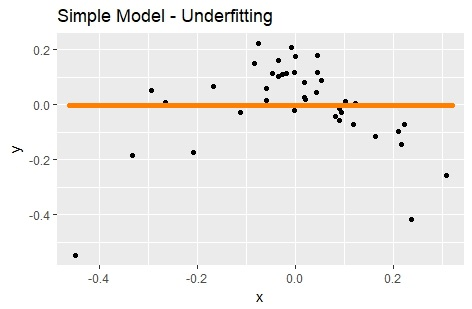
\includegraphics[scale=.5]{figs/plt_underfit.jpg}
        }
    \end{minipage}%
    \begin{minipage}{.5\linewidth}
        \centering
        \subfloat[A overfitting model]{
            \label{fig:overfit}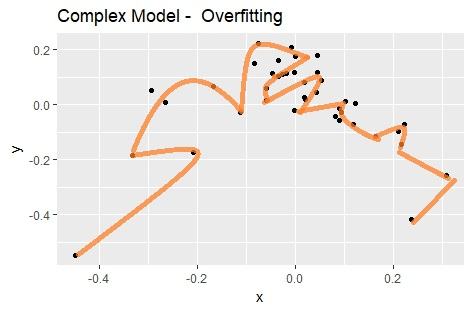
\includegraphics[scale=.5]{figs/plt_overfit.jpg}
        }
    \end{minipage}\par\medskip
    \centering
    \subfloat[The underlying model]{
        \label{main:c}
        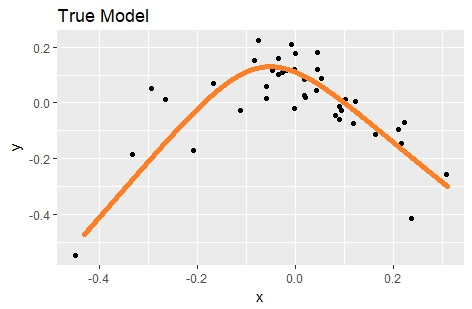
\includegraphics[scale=.5]{figs/plt_true.png}
        }
    \label{fig:main}
    \caption{Plots underfitting, overfitting, and underlying model
             from \cite{the-bias-variance-tradeoff}}
\end{figure}


\begin{figure}[!h]
    \centering
    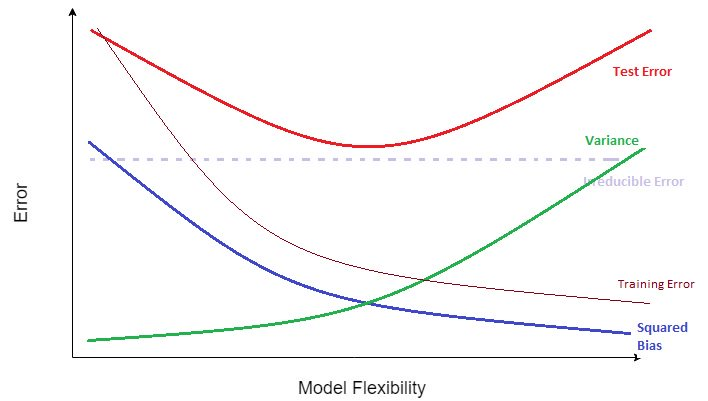
\includegraphics[width=0.8\textwidth]{figs/bias-var-trade.jpg}
    \caption{
        Plot the sq. bias, variance, training error, and test error
        from \cite{the-bias-variance-tradeoff}
    }
    \label{fig:bias-vars-tradeoff}
\end{figure}

% ---------------------------------------------------------------------
\pagebreak

\bibliographystyle{unsrt}
\bibliography{ref}
\end{document}
